\section{Mockup dell'applicazione}
Prima di realizzare l'app che permette all'utente di interagire con il servizio abbiamo pensato \ di creare dei mockup del design.
In questo modo la scrittura dell'applicazione può proseguire basandosi su un design concordato con tutto il team e l'eventuale committente.
Mettere a disposizione dei mockup e usarli per accordarsi sul design permette una progettazione più veloce e consistente rispetto alle modifiche fatte
più avanti nel tempo direttamente sul prodotto software.
Durante la realizzazione dell'app gli sviluppatori seguiranno al meglio i mockup, tuttavia alcune minime variazioni potrebbero emergere, per esempio a causa
di differenti elementi grafici messi a disposizione da Figma rispetto che da Flutter.

\begin{figure}
    \subsection{Homepage e Dettagli di un Evento}
    \fbox{\begin{subfigure}{0.47\textwidth}
        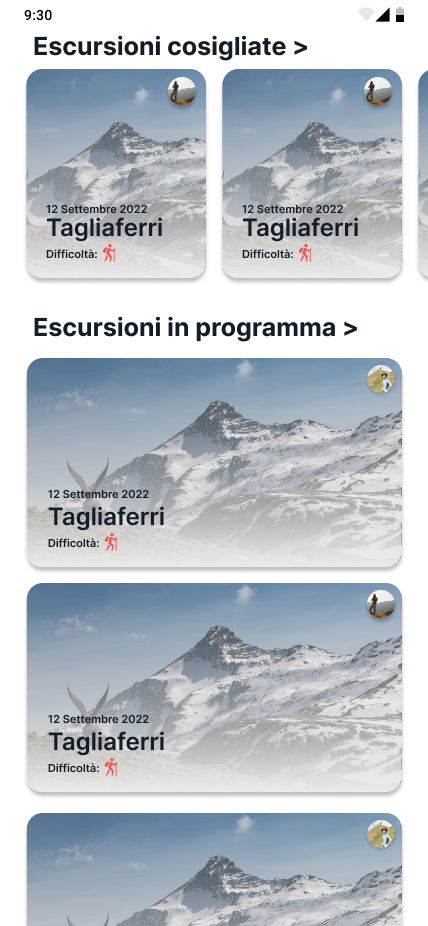
\includegraphics[width=\linewidth]{capitoli/asset/homepage.png}
        \caption{Homepage}
    \end{subfigure}}
    \hfill
    \fbox{\begin{subfigure}{0.47\textwidth}
        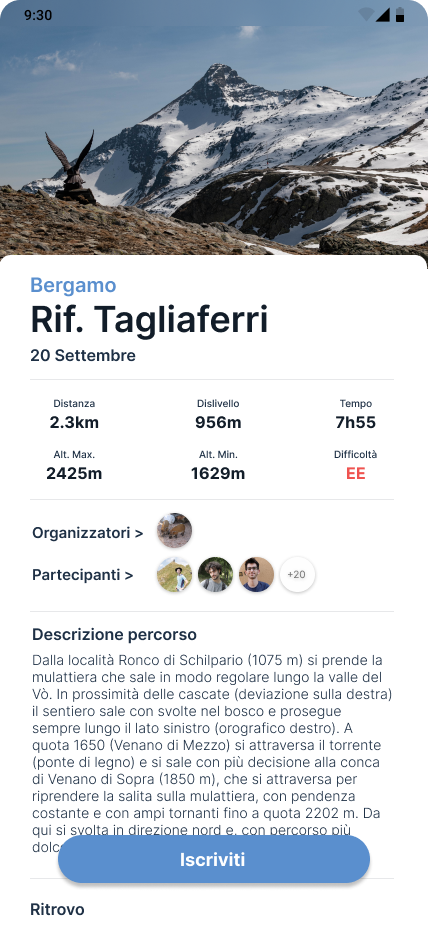
\includegraphics[width=\linewidth]{capitoli/asset/escursione.png}
        \caption{Dettagli di un evento}
    \end{subfigure}}
\end{figure}

\begin{figure}
    \subsection{Login e registraszione dell'utente}
    \fbox{\begin{subfigure}{0.47\textwidth}
        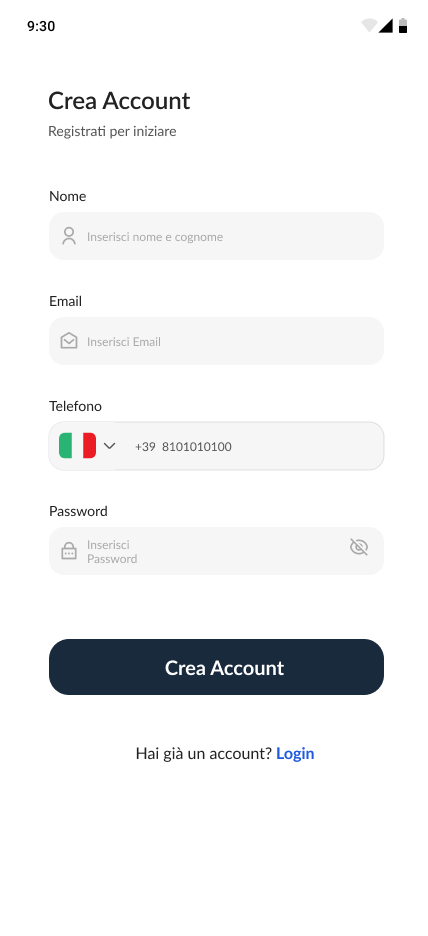
\includegraphics[width=\linewidth]{capitoli/asset/signupMail.png}
        \caption{Signup tramite mail}
    \end{subfigure}}
    \hfill
    \fbox{\begin{subfigure}{0.47\textwidth}
        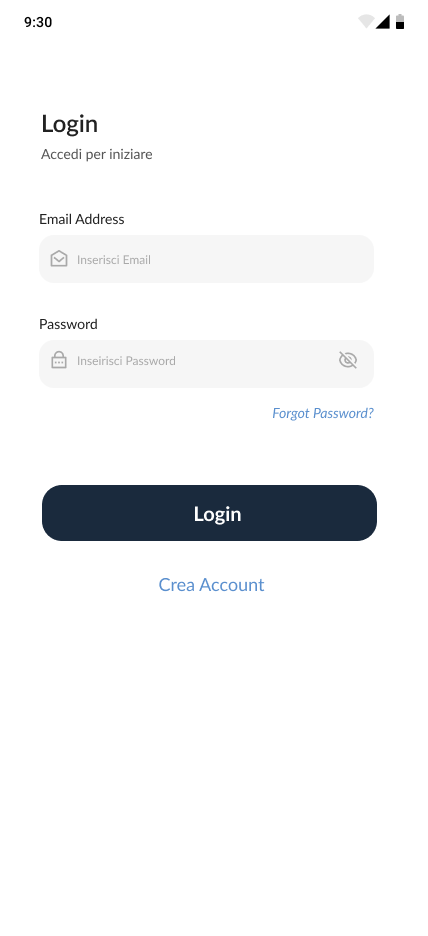
\includegraphics[width=\linewidth]{capitoli/asset/login.png}
        \caption{Login}
    \end{subfigure}}
\end{figure}

\begin{figure}
    \subsection{Ricerca escursione e Filtraggio}
    \fbox{\begin{subfigure}{0.47\textwidth}
        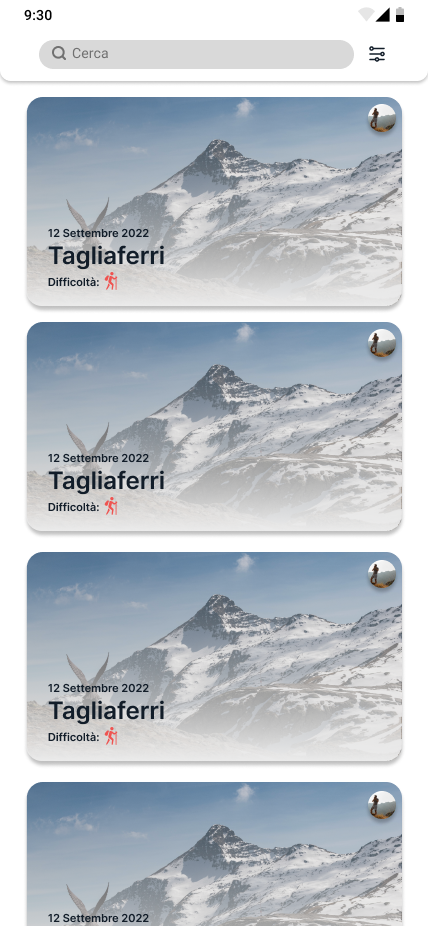
\includegraphics[width=\linewidth]{capitoli/asset/cerca.png}
        \caption{Ricerca di una escursione}
    \end{subfigure}}
    \hfill
    \fbox{\begin{subfigure}{0.47\textwidth}
        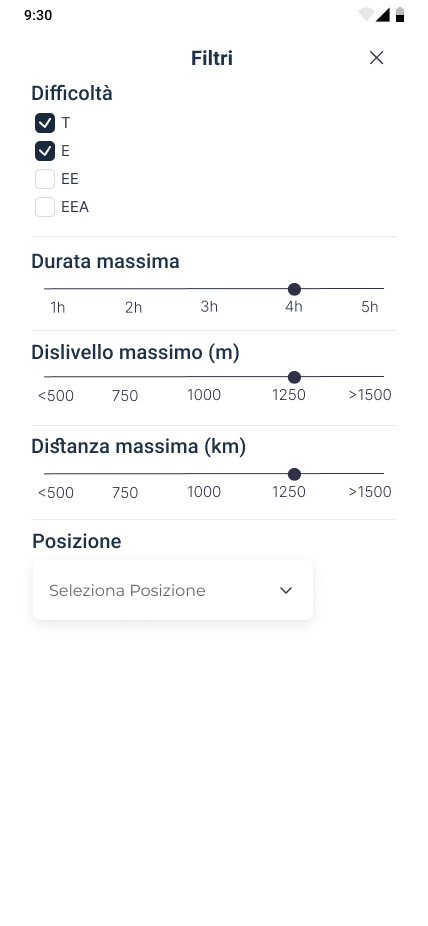
\includegraphics[width=\linewidth]{capitoli/asset/filtri.png}
        \caption{Filtraggio delle escursioni}
    \end{subfigure}}
\end{figure}

\begin{figure}
    \subsection{Visualizzazione del profilo utente}
    \fbox{\begin{subfigure}{0.47\textwidth}
        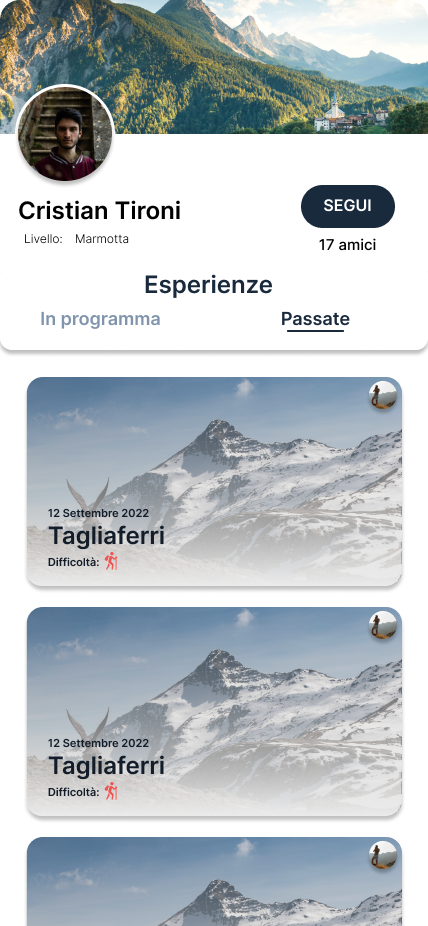
\includegraphics[width=\linewidth]{capitoli/asset/profiloUtente.png}
        \caption{Profilo utente normale}
    \end{subfigure}}
    \hfill
    \fbox{\begin{subfigure}{0.47\textwidth}
        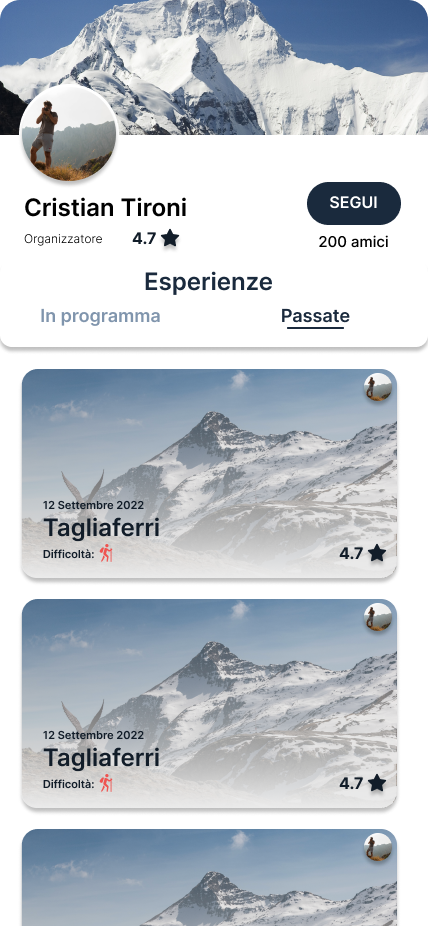
\includegraphics[width=\linewidth]{capitoli/asset/profiloOrganizzatore.png}
        \caption{Profilo organizzatore}
    \end{subfigure}}
\end{figure}